%http://pgfplots.sourceforge.net/gallery.html
\subsection{Mundo dos Blocos}\label{problemas:blocos}

O mundo dos blocos consiste de um conjunto de blocos, uma mesa e uma mão de robô. Os blocos podem ser empilhados ou estar em cima da mesa. Um bloco está \textbf{livre} se não há blocos em cima dele. Um bloco $A$ pode ser movido para cima de outro bloco $B$, se $B$ estiver livre. A mão robótica pode segurar um bloco ou estar livre.

Os blocos podem estar inicialmente em qualquer posição. O objetivo é encontrar um plano que move de uma configuração de blocos para outra.

A figura \ref{fig:blocos} mostra um exemplo de como seria um estado inicial e um estado final neste domínio.

\begin{figure}[H]%[htb]
  \centering
  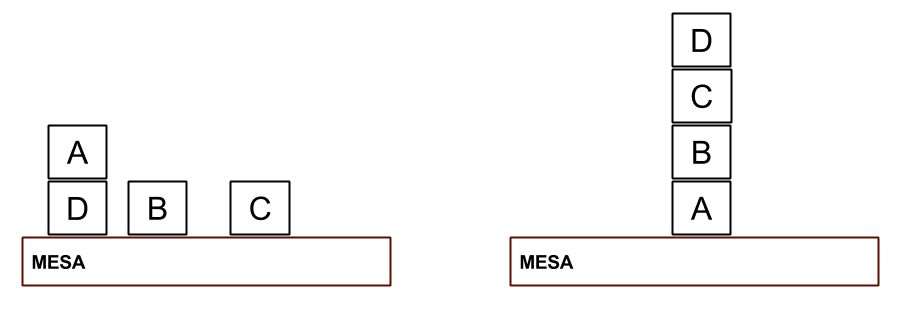
\includegraphics[width=10cm]{figures/blocos.png}
  \caption{Exemplo de estado inicial e final para o Mundo dos Blocos}
  \label{fig:blocos}
\end{figure}

Com o domínio do mundo dos blocos, fizemos trinta e cinco testes com um número de blocos de quatro até dezessete. Para cada número de blocos do problema, tínhamos três diferentes configurações de estado inicial e final.

\subsubsection{Resultados}\label{problemas:blocos:resultados}

%Grafico para time - Mundo dos blocos
\begin{figure}[H]
\centering
\begin{tikzpicture}
  \begin{axis}[
      only marks, xtick=data, xticklabels 
from table={plot/timeBlocos2.dat}{Problema},
      xticklabel style={rotate=90},
      axis lines=left,
      xlabel={Problemas do Mundo dos Blocos},
      xlabel style={at={(0.5,-0.05)}},
      ylabel={Tempo de Execução em milissegundos $log_{10}$},
      enlarge x limits={abs={0.0001*\pgfplotbarwidth}},
      legend style={at={(0.5,-0.20)},anchor=north,legend columns=1},
      height=9cm, width=15cm]

      \addplot table [x expr=\coordindex, y=H0]{plot/timeBlocos2.dat};
      \addplot table [x expr=\coordindex,
      y=GraphPlanHeuristic]{plot/timeBlocos2.dat};
      \addplot table [x expr=\coordindex, 
      y=GraphPlanHeuristicOpt]{plot/timeBlocos2.dat};
      \addplot table [x expr=\coordindex, 
      y=HSP_AddHeuristic]{plot/timeBlocos2.dat};
      \addplot table [x expr=\coordindex, 
      y=HSP_MaxHeuristic]{plot/timeBlocos2.dat};

  \legend{H0, Graph Plan, Graph Plan Otimo, HSP ADD, HSP MAX}
  \end{axis}
\end{tikzpicture}
\caption{Tempo de Execução - Mundo dos blocos}
\label{fig:timeBlocos}
\end{figure}
%%%%%%%%%%%%

Quanto ao tempo de execução, vemos na figura \ref{fig:timeBlocos} que a heurística HSPAdd foi a que melhor produziu resultados, conseguindo resolver problemas mais difíceis. Já o GraphPlan foi o que teve o pior comportamento: foi o que mais demorou para devolver uma solução e o que resolveu a menor quantidade de problemas.

%Grafico para nos Visitados - Mundo dos blocos
\begin{figure}[H]
\centering
\begin{tikzpicture}
  \begin{axis}[
      only marks, xtick=data, xticklabels 
from table={plot/visitadosBlocos.dat}{Problema},
      xticklabel style={rotate=90},
      axis lines=left,
      xlabel={Problemas do Mundo dos Blocos},
      xlabel style={at={(0.5,-0.05)}},
      ylabel={Número de nós Visitados ($log_{10}$)},
      enlarge x limits={abs={0.0001*\pgfplotbarwidth}},
      legend style={at={(0.5,-0.20)},anchor=north,legend columns=1},
      height=9cm, width=15cm]

      \addplot table [x expr=\coordindex, y=H0]{plot/visitadosBlocos.dat};
      \addplot table [x expr=\coordindex,
      y=GraphPlanHeuristic]{plot/visitadosBlocos.dat};
      \addplot table [x expr=\coordindex, 
      y=GraphPlanHeuristicOpt]{plot/visitadosBlocos.dat};
      \addplot table [x expr=\coordindex, 
      y=HSP_AddHeuristic]{plot/visitadosBlocos.dat};
      \addplot table [x expr=\coordindex, 
      y=HSP_MaxHeuristic]{plot/visitadosBlocos.dat};
  \legend{H0, Graph Plan, Graph Plan Otimo, HSP ADD, HSP MAX}
  \end{axis}
\end{tikzpicture}
\caption{Nós Visitados - Mundo dos blocos}
\label{fig:visitadosBlocos}
\end{figure}

A figura \ref{fig:visitadosBlocos} mostra que a heurística HSPAdd visitou o menor número de nós para todas os problemas. Já a heurística H0 foi a que visitou o maior número de nós. Isso já era esperado porque a H0 produz uma busca em largura no grafo.

%Nos gerados e visitados Blocos
\begin{table}[H]
\begin{tabular}{l|l|l|l|l|l|l|l|l|l|l|}
\cline{2-11}
                            & \multicolumn{2}{c|}{H0} & \multicolumn{2}{c|}{\begin{tabular}[c]{@{}c@{}}Graph \\ Plan\end{tabular}} & \multicolumn{2}{c|}{\begin{tabular}[c]{@{}c@{}}Graph \\ Plan \\ Optimo\end{tabular}} & \multicolumn{2}{c|}{\begin{tabular}[c]{@{}c@{}}HSP \\ ADD\end{tabular}} & \multicolumn{2}{c|}{\begin{tabular}[c]{@{}c@{}}HSP \\ MAX\end{tabular}} \\ \hline
\multicolumn{1}{|l|}{Prob.} & Visit.     & Ger.       & Visit.                               & Ger.                                & Visit.                                    & Ger.                                     & Visit.                              & Ger.                              & Visit.                              & Ger.                              \\ \hline
\multicolumn{1}{|l|}{4-0}   & 125        & 257        & 37                                   & 55                                  & 33                                        & 48                                       & 19                                  & 25                                & 38                                  & 53                                \\ \hline
\multicolumn{1}{|l|}{4-1}   & 110        & 224        & 30                                   & 46                                  & 27                                        & 42                                       & 22                                  & 32                                & 36                                  & 52                                \\ \hline
\multicolumn{1}{|l|}{4-2}   & 109        & 220        & 29                                   & 43                                  & 19                                        & 27                                       & 18                                  & 24                                & 32                                  & 44                                \\ \hline
\multicolumn{1}{|l|}{5-0}   & 732        & 1647       & 182                                  & 308                                 & 130                                       & 209                                      & 61                                  & 83                                & 119                                 & 167                               \\ \hline
\multicolumn{1}{|l|}{5-1}   & 796        & 1867       & 165                                  & 280                                 & 100                                       & 163                                      & 38                                  & 50                                & 110                                 & 152                               \\ \hline
\multicolumn{1}{|l|}{5-2}   & 866        & 2044       & 601                                  & 1198                                & 350                                       & 648                                      & 60                                  & 81                                & 124                                 & 173                               \\ \hline
\multicolumn{1}{|l|}{6-0}   & 4372       & 10363      & 335                                  & 590                                 & 123                                       & 187                                      & 110                                 & 145                               & 157                                 & 239                               \\ \hline
\multicolumn{1}{|l|}{6-1}   & 6601       & 17108      & 5411                                 & 11830                               & 373                                       & 585                                      & 69                                  & 91                                & 282                                 & 374                               \\ \hline
\multicolumn{1}{|l|}{6-2}   & 7057       & 18473      & 4822                                 & 10137                               & 3143                                      & 6555                                     & 105                                 & 137                               & 409                                 & 568                               \\ \hline
\multicolumn{1}{|l|}{7-0}   & 54696      & 149861     & 28867                                & 57943                               & 3394                                      & 5865                                     & 122                                 & 159                               & 2035                                & 3154                              \\ \hline
\multicolumn{1}{|l|}{7-1}   & 65990      & 185278     & 55370                                & 133602                              & 25511                                     & 55594                                    & 216                                 & 277                               & 2213                                & 3557                              \\ \hline
\multicolumn{1}{|l|}{7-2}   & 64676      & 181625     & 38891                                & 82129                               & 21759                                     & 45321                                    & 127                                 & 183                               & 2808                                & 4358                              \\ \hline
\multicolumn{1}{|l|}{8-0}   & 641879     & 1915788    & -1                                   & -1                                  & 43151                                     & 78721                                    & 210                                 & 256                               & 11498                               & 19168                             \\ \hline
\end{tabular}
\caption{Nós Visitados e Gerados - Mundos dos Blocos}
\label{tab:nosBlocos}
\end{table}

A tabela \ref{fig:custoBlocos} apresenta os nós visitados e gerados para todas as heurísticas usadas. Valores -1 significam que o problema não terminou de ser resolvido. Ressaltamos que a otimização feita no GraphPlan resultou em menor número de nós visitados e gerados. Porém, o HSPAdd foi a heurística que apresentou melhores resultados nesses quesitos.

%Grafico para custo - Mundo dos blocos
\begin{figure}[H]
\centering
\begin{tikzpicture}
  \begin{axis}[
      only marks, xtick=data, xticklabels 
from table={plot/custoBlocos.dat}{Problema},
      xticklabel style={rotate=90},
      axis lines=left,
      xlabel={Problemas do Mundo dos blocos},
      xlabel style={at={(0.5,-0.05)}},
      ylabel={Custo da Solução},
      enlarge x limits={abs={0.0001*\pgfplotbarwidth}},
      legend style={at={(0.5,-0.20)},anchor=north,legend columns=1},
      height=9cm, width=15cm]

      \addplot table [x expr=\coordindex, y=H0]{plot/custoBlocos.dat};
      \addplot table [x expr=\coordindex,
      y=GraphPlanHeuristic]{plot/custoBlocos.dat};
      \addplot table [x expr=\coordindex, 
      y=GraphPlanHeuristicOpt]{plot/custoBlocos.dat};
      \addplot table [x expr=\coordindex, 
      y=HSP_AddHeuristic]{plot/custoBlocos.dat};
      \addplot table [x expr=\coordindex, 
      y=HSP_MaxHeuristic]{plot/custoBlocos.dat};
  \legend{H0, Graph Plan, Graph Plan Otimo, HSP ADD, HSP MAX}
  \end{axis}
\end{tikzpicture}
\caption{Custo da Solução - Mundo dos blocos}
\label{fig:custoBlocos}
\end{figure}

Por fim, em relação ao custo da solução, a figura \ref{fig:custoBlocos} mostra que, para as primeiras instâncias do problema, as heurísticas empatam. Já para instâncias maiores, o GraphPlan otimizado e a H0 apresentam as soluções com menor custo.